\section{Detailed image processing methods}
\label{sec:A}

Four red-green-blue (RGB) color images (\fref{fig:app:images}) were taken using a Samsung S8 smartphone camera: (1) the orange construction paper with the metal rigid physical model of a single leaf; (2) the orange construction paper alone; (3) the fan aperture alone with black construction paper mask on a blue background; and (4) the fan aperture obstructed by the live \Cxparadisi\ grapefruit specimen. Black and orange construction paper were chosen to maximize contrast and allow easy automatic color segmentation. 
\begin{figure}
\begin{center}
%\includegraphics[width=0.49\columnwidth]{figures/MetalLeaf.jpg}
%\includegraphics[width=0.49\columnwidth]{figures/Paper.jpg} \\
%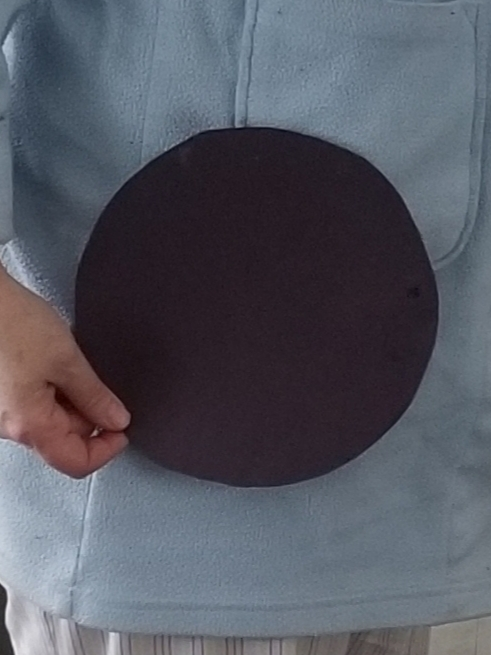
\includegraphics[width=0.49\columnwidth]{figures/Fan1.jpg}
%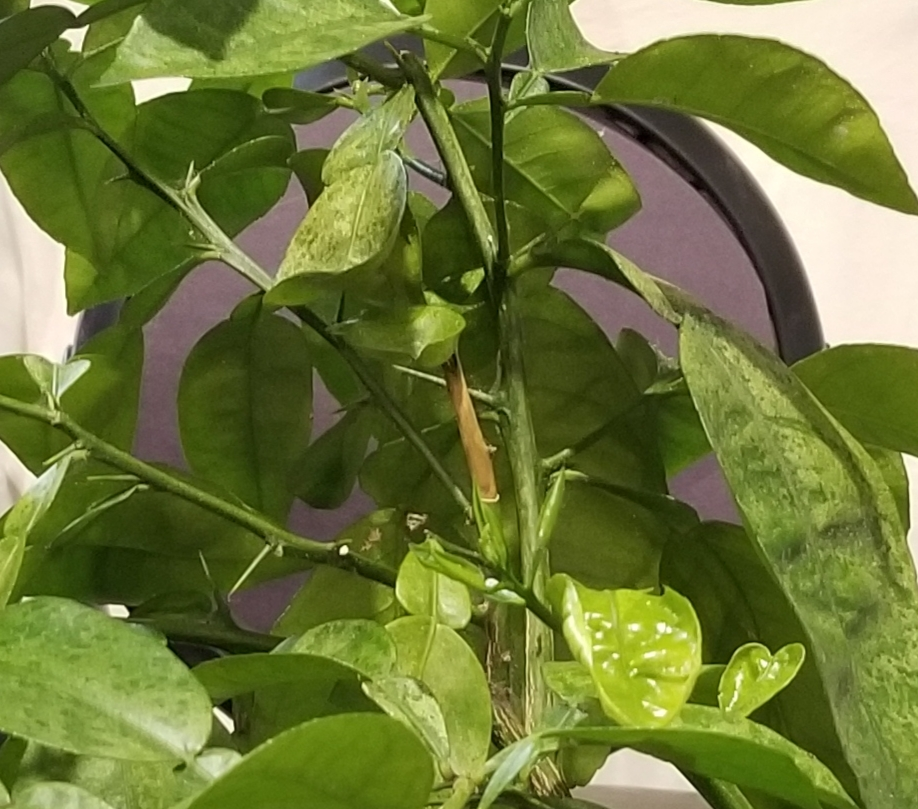
\includegraphics[width=0.49\columnwidth]{figures/Fan.jpg}
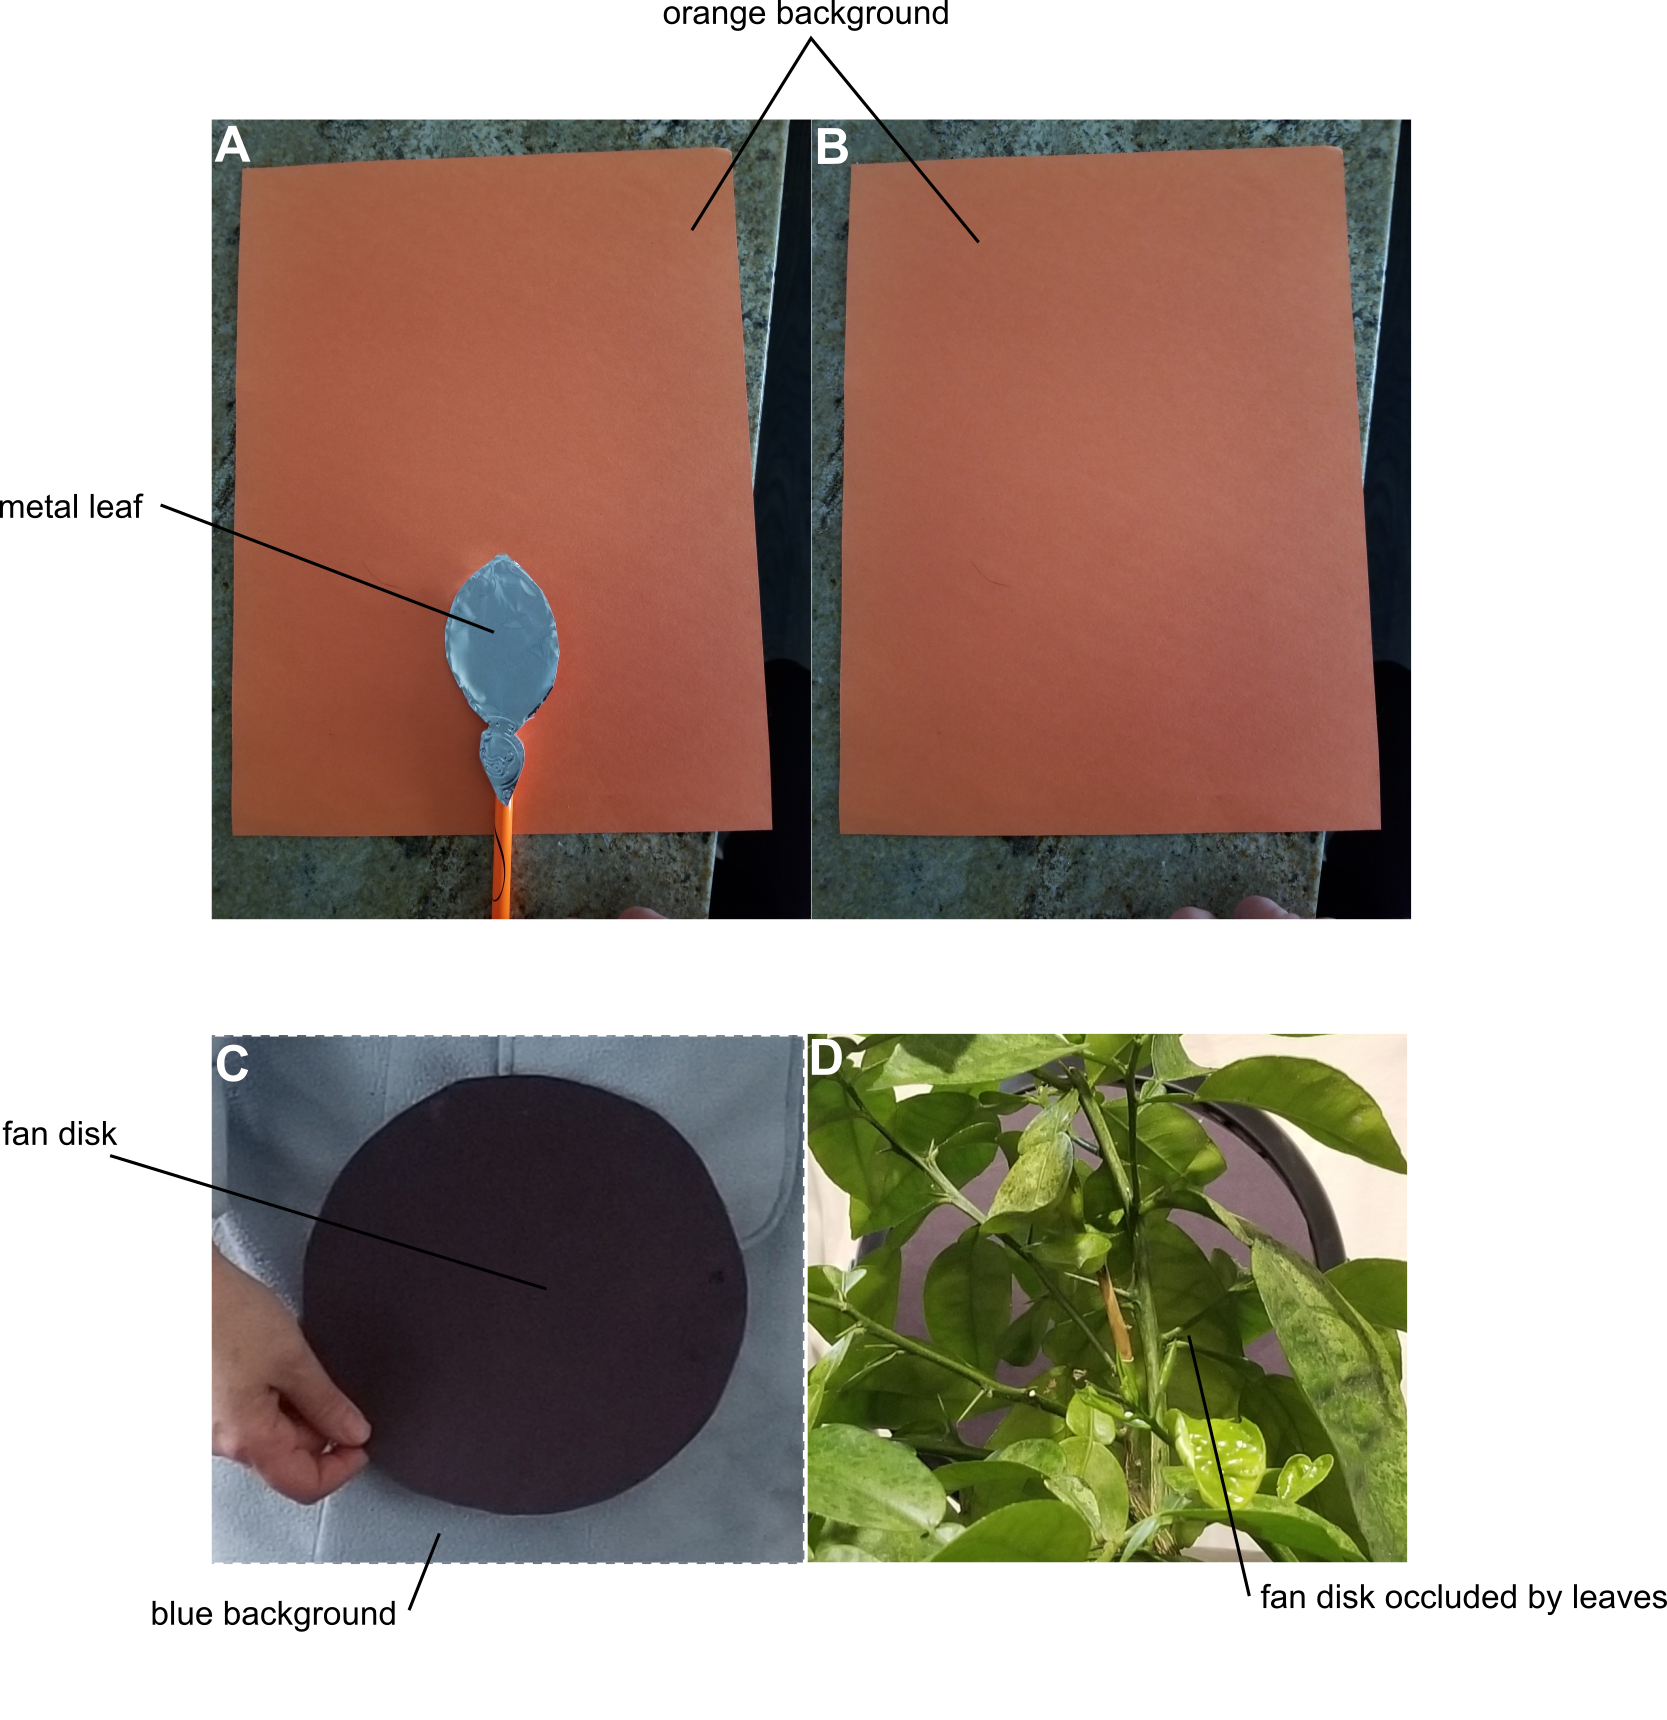
\includegraphics{figures/fig7.png}
\end{center}
\caption{(A) Metal rigid physical model of a leaf on orange background; (B) orange background; (C) fan aperture; (D) fan aperture obstructed by the live \Cxparadisi\ specimen.}
\label{fig:app:images}
\end{figure}


\subsection{Color blob detection/segmentation using \Matlab}
Color blob detection/segmentation was obtained using the \lstinline{colorThresholder} tool in \Matlab. Images were first converted from RGB colorspace to hue-saturation-value (HSV) colorspace; thresholding was then applied in each channel using the sliders to obtain a binary image corresponding to (1) the area of the orange sheet obstructed by the metal leaf; (2) the orange sheet; (3) the fan; (4) the area of the fan obstructed by the plant, respectively. 

\subsection{Area calculation}
The binary images were labeled as contiguous regions using the \lstinline{bwlabel} command; the largest blobs were manually selected for futher processing. From the labeled region, the \lstinline{regionprops} command was used to obtain the \lstinline{FilledArea} property, which corresponds to the number of pixels contained in the selected blob. 

Using known dimensions of the paper, the area of leaves could be found by calculating the ratio of exposed to unexposed paper area. In the case of the orange construction paper, the paper physical dimensions were \SI{9x12}{\inch} (\SI{0.229x0.305}{\meter}). In the case of the fan, the disk area was \SI{8.5}{\inch} (\SI{0.216}{\meter}) in diameter; these provided the scaling between pixel area and physical area:
\begin{lstlisting}
paperarea=9*12/144;
blackarea=8.5^2*pi/(4*144);
metalarea=leafsize.FilledArea/papersize.FilledArea*paperarea;
grapefruitarea=blackarea-blackarea*fansize/fan1size.FilledArea;
\end{lstlisting}

Area analysis code is provided in the file \lstinline{data/matlab/Calculating Areas.m} in the Github repository at:\\ \url{https://github.com/ew282d-evangelista/ew282d-sp2020-0451-smith}. 



